\documentclass[sigconf]{acmart}

% ACM-compatible mathematical and algorithm typesetting.
\usepackage{amsmath}
\usepackage{algorithm}
\usepackage{algorithmic} % ACM-listed algorithm package
\usepackage{pgfplots}
\pgfplotsset{compat=1.17}

\setcopyright{none}
\copyrightyear{}
\acmISBN{}
\acmDOI{}
\settopmatter{printacmref=true}
\acmYear{2026}
\acmConference[TRTDMC '26]
{6th TU/e Research Topics on Data Mining Conference}
{2026}
{Eindhoven, The Netherlands}

% Shorthand for expressions used frequently in the existing manuscript.
\newcommand{\ICV}{\operatorname{ICV}}
\newcommand{\PICV}{\operatorname{PICV}}
\newcommand{\TSS}{\operatorname{TSS}}
\newcommand{\surp}{\operatorname{surp}}
\newcommand{\supp}{\operatorname{supp}}
\newcommand{\disc}{\mathrm{disc}}
\newcommand{\pool}{\mathrm{pool}}
\newcommand{\Freq}{\mathrm{Freq}}
\newcommand{\Len}{\mathrm{Len}}

\begin{document}

\title{Interactive Pattern Mining with Multiple Complementary Dynamic Features}

\author{Evi Levels}
\affiliation{\institution{Eindhoven University of Technology}\department{Department of Mathematics and Computer Science}\city{Eindhoven}\country{The Netherlands}}
\author{Paula de la Hoz M\'endez}
\affiliation{\institution{Eindhoven University of Technology}\department{Department of Mathematics and Computer Science}\city{Eindhoven}\country{The Netherlands}}
\author{Alicja Ksi\k{a}żkiewicz }
\affiliation{\institution{Eindhoven University of Technology}\department{Department of Mathematics and Computer Science}\city{Eindhoven}\country{The Netherlands}}
\author{Miguel Ramirez}
\affiliation{\institution{Eindhoven University of Technology}\department{Department of Mathematics and Computer Science}\city{Eindhoven}\country{The Netherlands}}
\author{Cristian Ni\c{t}\u{a}}
\affiliation{\institution{Eindhoven University of Technology}\department{Department of Mathematics and Computer Science}\city{Eindhoven}\country{The Netherlands}}

\begin{abstract}
Interactive pattern mining learns a user's preferences from rankings of a few patterns at a time.
\textsc{DiSPaLe} captures interactions between items by adding, at every iteration, the sub-pattern that best
discriminates the user's ranking as a temporary feature, whose learned weight is then folded into the item
weights. We study whether selecting several complementary discriminant sub-patterns per iteration improves
the learned preferences. We extend \textsc{DiSPaLe} with five selection rules, including a partition-gain
criterion that rewards sub-patterns separating groups the others cannot, and introduce a simulated user whose
preference consists of independent item combinations. We also correct six errors in the published
implementation and verify that undoing them reproduces it exactly. On three datasets, no selection rule
improves the model as long as the sub-pattern features are folded into item weights, since the folded model
cannot represent combinations of items. Keeping the selected sub-patterns as permanent features improves the
learned model significantly, and selecting several of them per iteration adds a further, smaller gain at no
measurable cost.
\end{abstract}

\ccsdesc[500]{Information systems~Data mining}
\keywords{interactive pattern mining, preference learning, discriminant sub-patterns, dynamic features}
\maketitle

\section{Introduction}
Pattern mining aims to discover meaningful patterns in large datasets. However, traditional approaches often generate a large number of patterns from which only a small number may be relevant to a particular user. Since interestingness depends on the user's preferences, interactive pattern mining incorporates user feedback into the mining process rather than relying only on predefined rules. Nevertheless, learning these preferences remains a challenging task when they depend on interactions between items rather than on individual pattern features. 

DiSPaLe addresses this limitation by identifying discriminating sub-patterns from the user's rankings and incorporating them as temporary dynamic features. These features allow the ranking model to capture interactions between items without permanently increasing the feature space. However, the original algorithm selects only the sub-pattern with the highest Inter-Class Variance (ICV) at each iteration. This may be insufficient when the user's preferences depend on several distinct item combinations. Moreover, simply selecting multiple high-ICV sub-patterns may introduce redundancy, as different sub-patterns can explain essentially the same preference. 

In this paper, we investigate whether selecting multiple complementary discriminating sub-patterns can improve the preference learning in interactive pattern mining. We extended DiSPaLe to extract multiple candidates and investigate different selection strategies that account for their discriminating and complementarity abilities. We also adapt the dynamic feature representations and weight updates to accommodate multiple sub-patterns. To evaluate the proposed approach, we introduced a simulated user whose preferences depend on several item combinations, allowing us to compare the extended algorithm against the corrected original DiSPaLe implementation. Finally, since the folded model can only represent item weights, we also evaluate keeping the selected sub-patterns as permanent features.


\section{Literature Study}
\label{sec:literature}

\paragraph{Interestingness and redundancy.}
Pattern mining typically returns far more patterns than a user can inspect, only a few of which are interesting to that user~\cite{xin2006}. Objective interestingness measures~\cite{geng2006} capture general properties of a pattern, such as how surprising its frequency is, but not the goals of a particular analyst, and choosing and combining them requires data-mining expertise that domain experts often lack~\cite{dzyuba2014}. A first line of work therefore condenses the output into small sets of non-redundant patterns. Redundancy-aware top-$k$ mining trades the significance of each pattern against its overlap with the others~\cite{xin2006redundancy}, Krimp selects the itemsets that best compress the data~\cite{vreeken2011}, and diverse subgroup set discovery avoids returning many variations of the same subgroup~\cite{vanleeuwen2012}. These methods rely on general selection principles that we also use: maximal marginal relevance, which discounts relevance by similarity to what was already chosen~\cite{carbonell1998}, and greedy maximisation of monotone submodular objectives, which is guaranteed to reach a fraction $1-1/e$ of the optimum~\cite{nemhauser1978}. All of them, however, select \emph{result} patterns once, against a fixed objective.

\paragraph{Interactive pattern mining.}
A second line of work lets the user steer the mining. Xin et al.\ learn a user's prior knowledge from feedback on mined patterns to re-rank the remaining ones~\cite{xin2006}, Rüping learns to rank subgroups from user preferences~\cite{rueping2009}, Bhuiyan et al.\ sample frequent patterns with a Markov chain that is updated with the user's feedback~\cite{bhuiyan2012}, and One Click Mining infers preferences implicitly from the user's interaction~\cite{boley2013}. Dzyuba et al.~\cite{dzyuba2014} cast the problem as learning a ranking function over patterns from pairwise preferences, with pairwise learning to rank~\cite{joachims2002,furnkranz2010}. LetSIP~\cite{dzyuba2017} combines this learner, a logistic model trained by $L_1$-regularised stochastic coordinate descent~\cite{shalevshwartz2011}, with Flexics, which samples each query from the frequent patterns in proportion to the current ranking function~\cite{dzyuba2017}, building on earlier work on pattern sampling~\cite{boley2011,hasan2009}. The interaction loop of LetSIP is the basis of \textsc{DiSPaLe} and of our extension.

\paragraph{Pattern features.}
These approaches describe a pattern by simple and mostly independent descriptors, such as the items it contains, its length or its frequency. A linear ranking function over such descriptors cannot express preferences that depend on interactions between items, for instance a user who prefers pattern $A$ when $B$ is also present but not when $C$ is. Hien et al.\ therefore exploit more complex pattern features~\cite{hien2022}, and \textsc{DiSPaLe}~\cite{hien2023} constructs them during the interaction: at every iteration, it selects the sub-pattern whose presence best separates highly ranked from poorly ranked patterns, measured by the inter-class variance (ICV)~\cite{morishita2000}, adds it as a temporary dynamic feature, and folds its learned weight into the base feature weights before discarding it. This captures item interactions without permanently increasing the feature space.

\paragraph{Research gap.}
\textsc{DiSPaLe} selects only the single sub-pattern with the highest ICV, which may be insufficient when a user's preferences depend on several distinct combinations of items, for example a user who prefers patterns containing $\{A,B\}$ and, independently, patterns containing $\{C,D\}$. Several discriminant sub-patterns could capture more of such a preference, but simply taking the $m$ highest-ICV sub-patterns tends to return redundant ones such as $\{A,B\}$, $\{A,B,C\}$ and $\{A,B,D\}$. Redundancy-aware selection is well studied for the patterns presented to a user, but, to our knowledge, not for the features from which an interactive learner builds its model. This leads to our research question: \emph{Can preference learning in interactive pattern mining be improved by selecting multiple complementary discriminant sub-patterns as dynamic features instead of only the strongest discriminant sub-pattern?}

\section{Preliminaries}
The original DiSPaLe algorithm~\cite{hien2023} follows the iterative interaction loop shown in Algorithm~\ref{alg:dispale}. It maintains a ranking function based on a weighted set of pattern features, whose weights the paper initialises to zero. At each iteration, the highest-ranked patterns from the previous query are retained, and new patterns are sampled according to the current ranking function. The user ranks the resulting query, and this feedback is added to the rankings collected over previous iterations. DiSPaLe builds on LetSIP~\cite{dzyuba2017}, which follows the same loop with the base features only, and samples each query with Flexics~\cite{dzyuba2017}, which draws frequent patterns with probability proportional to the current ranking function. 

DiSPaLe then searches for a discriminating sub-pattern that best explains the user's ranking. For each candidate sub-pattern, the query patterns are divided into two groups depending on whether they contain it. The difference between the mean ranks of these groups is measured using the Inter-Class Variance (ICV), and the sub-pattern with the highest ICV is selected. This sub-pattern is used to construct three dynamic features representing its presence, frequency in the datasets, and relative length. These features allow the preference learner to capture interactions between items that cannot be represented by the original features independently. 

The weights of the dynamic features are learned together with the base feature weights using the accumulated user feedback. The learned dynamic weights are then incorporated into the base feature weights, after which the temporary features are discarded. The updated weights are used to construct the ranking function for the next iteration, allowing the sampling process to progressively adapt to the user's preferences without permanently increasing the feature space. However, only one discriminating sub-pattern is selected at each iteration, which is the main limitation addressed by our extension.

\subsection{Corrections to the original code}
\label{subsec:corrections_to_code}
\paragraph{Corrections to the interaction loop.}
While re-implementing the extension we found that the publicly available DiSPaLe code does not execute Algorithm~\ref{alg:dispale} as written. First, the ranking function learned at the end of each iteration (line~11) was assigned to a local variable that went out of scope, so every query $\mathcal X^t$ was drawn with the initial weights $w_F^0$ instead of $\phi^{t-1}$: the learned model never influenced which patterns were shown to the user. We pass $\phi^t$ to the next call of \textsc{SamplePatterns}; the sampler itself (Flexics) is unchanged and only receives different weights. Second, \textsc{LearnWeights} resumed SCD from the inner products $w\cdot x$ of the previous iteration, although the dynamic features had been added and the weights folded since they were computed, so its gradients were wrong from the second iteration on; we recompute them. Third, \textsc{UpdateWeights} read the learned dynamic weight at the index given by the number of feature \emph{types} instead of after the base features, and therefore folded the weight of an unrelated item (item~$1$) instead of that of the sub-pattern. Finally, the code initialises all weights to $1$, not to $w_F^0=0$ as stated in the paper (line~5). With binary item features, the initial score of a pattern is then its length. We keep this initialisation, since starting from $0$ performs clearly worse (Table~\ref{tab:fidelity}). With these corrections, the loop structure of Algorithm~\ref{alg:dispale} is unchanged: our extension only modifies \textsc{MineDiscriminating}, \textsc{LearnWeights}, and \textsc{UpdateWeights} (lines 8--10).

\paragraph{Corrections to the sub-pattern search.}
We also corrected three errors in the original implementation of \textsc{MineDiscriminating}. First, the mean ranks in Eq.~(\ref{eq:icv}) were stored as integers, so every mean was rounded down and the ICV of many sub-patterns was wrong; we compute them as real numbers. Second, the cover of a longer sub-pattern $Y\cup\{i\}$ was computed by intersecting the stored cover of $Y$ in place, which overwrote the cover of $Y$; every further extension of $Y$ was then evaluated on a cover that was too small, so the ICV of longer sub-patterns could be wrong and the selected sub-pattern could differ from the true maximum. We intersect a copy of the cover instead. Third, a sub-pattern reachable from several shorter ones (e.g., $\{a,b\}$ from both $\{a\}$ and $\{b\}$) was evaluated once per parent. This only cost time when a single sub-pattern was kept, but would insert duplicate candidates into $C$, so we evaluate each sub-pattern once. Each of the six corrections can be undone individually. With all of them undone, our implementation reproduces a run of the published code exactly: the same queries, the same sub-patterns and the same learned weights at every iteration. Smaller fixes that do not affect our setting (an item index that is wrong when items are not the first feature type, stored pairs that could only grow by one feature, and two launcher options) are documented with the code.

\begin{algorithm}[tb]
\caption{DiSPaLe (Discriminating Sub-Pattern feature Learning)}\label{alg:dispale}
\footnotesize
\begin{algorithmic}[1]
\REQUIRE Dataset $D$, patterns $\mathcal X$; query size $k$, steps $T$, range $A$, retention $\ell$, feature representations $F$
\ENSURE Ranking function $\phi$
\STATE $U\gets\varnothing$; $w_F^0\gets0$; $\mathcal X^0\gets\varnothing$
\STATE $\phi^0\gets\phi_{\mathrm{logistic}}(w_F^0,A)$
\FOR{$t=1,\ldots,T$}
  \STATE $\mathcal X^t\gets\operatorname{Top}(\mathcal X^{t-1},\ell)$
  \STATE \hspace{1.35em}$\cup\operatorname{SamplePatterns}(D,\phi^{t-1},k-\ell)$
  \STATE $\hat R^t\gets\operatorname{Rank}(\mathcal X^t)$
  \STATE $\disc\gets\operatorname{MineDiscriminating}(\mathcal X^t,\hat R^t)$
  \STATE $U\gets U\cup\hat R^t$
  \STATE $(w_F^t,w_{F_{\disc}}^t)\gets\operatorname{LearnWeights}(U,F\cup F_{\disc})$
  \STATE $w_F^t\gets\operatorname{UpdateWeights}(w_F^t,w_{F_{\disc}}^t)$
  \STATE $\phi^t\gets\phi_{\mathrm{logistic}}(w_F^t,A)$
\ENDFOR
\STATE \textbf{return} $\phi^T$
\end{algorithmic}
\end{algorithm}

\section{Proposed Methodology}
We keep the original DiSPaLe Algorithm~\ref{alg:dispale} unchanged; our extension changes \textsc{MineDiscriminating} to return a set of $m$ sub-patterns, and \textsc{LearnWeights} / \textsc{UpdateWeights} to handle one set of features per sub-pattern. The only exception is the keep scheme of Section~\ref{subsec:keep}, which skips \textsc{UpdateWeights}.

\subsection{Simulated users}
\label{subsec:users}
As in the original DiSPaLe evaluation, the user's feedback is simulated by a ranking function that orders the $k$ patterns of each query. The implementation already provided three such users. The \emph{surprisingness user} (the default in the original experiments) scores a pattern by how much more frequently it occurs than its items independently, $\surp(X)=\max\{0,\supp(X)/|D|-\prod_{i\in X}p(i)\}$, where $p(i)$ is the relative frequency of item $i$. The \emph{frequency user} ranks the patterns by support. The \emph{Gaussian user} draws one random weight per item and scores a pattern by the sum of the weights of its items, multiplied by its support.

None of these users suits our research question. The Gaussian user's preference is additive over items, so a linear model on item features can already represent it, and sub-pattern features have nothing to add. The surprisingness and frequency users depend on global statistics of the pattern instead of on specific item combinations, so there is no ground truth for which sub-patterns explain their rankings, and we cannot check whether the selected sub-patterns are the right ones.

We therefore introduce a \emph{combination user} whose preference consists of several independent item combinations. The user is given a set of combinations $\mathcal S=\{(S_1,\omega_1),\ldots,(S_c,\omega_c)\}$, where each $S_j$ is a small itemset and $\omega_j$ its weight (negative for combinations the user dislikes). A pattern earns $\omega_j$ for every combination it contains:
\begin{equation}\label{eq:combination}
 u(X)=\sum_{j=1}^{c}\omega_j\mathbf{1}[S_j\subseteq X]+\varepsilon\,\surp(X),\quad \varepsilon=0.01.
\end{equation}
Combinations contribute additively, so a pattern containing several of them is preferred over one containing only one; within a combination, the reward is only earned when all its items are present. Since $\surp(X)\leq1$, the second term orders only patterns that contain the same combinations, provided that the distinct values of the first term differ by more than $\varepsilon$, as they do for unit weights. This within-combination interaction cannot be represented exactly by a linear model on single items. It also has a known ground truth, since the combinations $S_j$ are exactly the complementary sub-patterns our selection rules should recover. Algorithm~\ref{alg:combo} gives the ranking procedure.

\begin{algorithm}[tb]
\caption{ComboRank: ranking by the combination user}\label{alg:combo}
\footnotesize
\begin{algorithmic}[1]
\REQUIRE Query $\mathcal X^t=\{X_1,\ldots,X_k\}$, dataset $D$; combinations $\mathcal S=\{(S_j,\omega_j)\}_{j=1}^{c}$, tie-break $\varepsilon$
\ENSURE Ranking $\hat R^t$ of the query
\FOR{$i\in I$}
 \STATE $p(i)\gets |\{T\in D:i\in T\}|/|D|$
\ENDFOR
\FOR{$X\in\mathcal X^t$}
  \STATE $u(X)\gets0$
  \FOR{$(S_j,\omega_j)\in\mathcal S$}
    \IF{$S_j\subseteq X$} \STATE $u(X)\gets u(X)+\omega_j$ \ENDIF
  \ENDFOR
  \STATE $\surp(X)\gets\max\{0,\supp(X)/|D|-\prod_{i\in X}p(i)\}$
  \STATE $u(X)\gets u(X)+\varepsilon\surp(X)$
\ENDFOR
\STATE $\hat R^t\gets\operatorname{sort}_{\mathrm{decreasing}\ u}(\mathcal X^t)$
\STATE \textbf{return} $\hat R^t$
\end{algorithmic}
\end{algorithm}

\paragraph{Running example.}
We follow one iteration of a real run on the soybean dataset with $k=10$ and a combination user who likes $\{29,37\}$ (\texttt{stem\_cankers=absent}, \texttt{external\_decay=absent}) and $\{33,45\}$ (\texttt{canker\_lesion=dna}, \texttt{sclerotia=absent}). Table~\ref{tab:ex_query} shows the first query in the order the user ranks it. The three patterns that contain $\{33,45\}$ score $1$ plus a small surprisingness term and come first; the seven others contain no liked pair and are ordered by surprisingness alone. Since all weights start at $1$, the model score $w\cdot x$ of every pattern is its length.

\begin{table}[t]
\centering
\caption{Running example: the first query, ranked by the user (rank $0$ preferred). \#: position in the sampled order; liked pair in bold.}
\label{tab:ex_query}
\small
\setlength{\tabcolsep}{4pt}
\begin{tabular}{rrlrr}
\toprule
Rank & \# & Pattern & $w\cdot x$ & $u(X)$ \\
\midrule
0 & 3 & $\{8,11,27,29,\mathbf{33},40,42,\mathbf{45}\}$ & 8 & 1.0008 \\
1 & 6 & $\{19,\mathbf{33},42,\mathbf{45},47\}$          & 5 & 1.0003 \\
2 & 7 & $\{7,13,18,27,\mathbf{33},\mathbf{45}\}$        & 6 & 1.0002 \\
3 & 5 & $\{11,26,28,32,40\}$                            & 5 & 0.0012 \\
4 & 4 & $\{11,13,28,35,40,42,45\}$                      & 7 & 0.0007 \\
5 & 1 & $\{4,7,23,26,40,45\}$                           & 6 & 0.0004 \\
6 & 9 & $\{10,20,35,40,42\}$                            & 5 & 0.0003 \\
7 & 8 & $\{11,13,23,26,34,40,47\}$                      & 7 & 0.0003 \\
8 & 2 & $\{14,18,27,37,40,42,47\}$                      & 7 & 0.0003 \\
9 & 0 & $\{7,11,23,32,37,40,45\}$                       & 7 & 0.0000 \\
\bottomrule
\end{tabular}
\end{table}

\subsection{Mining multiple discriminating sub-patterns}
In DiSPaLe, \textsc{MineDiscriminating} (Algorithm 3 of the original paper) returns a single sub-pattern: the one with the highest inter-class variance (ICV) between the ranks of the query patterns that contain it and the ranks of those that do not. With ranks $r(X)\in\{0,\ldots,k-1\}$ ($0$ being the most preferred) and $\mu=(k-1)/2$,
\begin{equation}\label{eq:icv}
\ICV(Y,\hat R)=|C_Y|(\mu-\bar r_{C_Y})^2+|\overline C_Y|(\mu-\bar r_{\overline C_Y})^2,
\end{equation}
where $C_Y=\{X\in\mathcal X:Y\subseteq X\}$ is the cover of $Y$ in the query, $\overline C_Y=\mathcal X\setminus C_Y$, and $\bar r$ denotes the mean rank of a group. Every time a sub-pattern matches or exceeds the current maximum, the previous one is discarded, so no second-best candidate is ever kept.

\paragraph{Running example (cont.).}
In Table~\ref{tab:ex_query}, $\mu=4.5$. The liked pair $Y=\{33,45\}$ is contained in the patterns of ranks $0,1,2$, so
\begin{equation*}
 \ICV(Y)=3\,(4.5-1)^2+7\,(4.5-6)^2=36.75+15.75=52.5,
\end{equation*}
the highest among the $39$ candidates with a positive ICV (sub-itemsets with the same cover counted once, see below). Next come $\{33,42,45\}$ (ranks $0,1$) and $\{37,40\}$ (ranks $8,9$), both with ICV $40.0$.

We change the procedure in two ways (Algorithm~\ref{alg:extract}). First, every sub-pattern with a positive ICV is kept as a candidate rather than overwritten. Second, once the search is complete, the candidates are sorted by decreasing ICV, with ties going to the longer sub-pattern as in the original implementation, and a selection rule \textsc{Select} returns at most $m$ of them. Since every selection rule starts from the first candidate in this order, $m=1$ yields the original DiSPaLe sub-pattern. Note that the original pseudocode only extends improving sub-patterns, while the original implementation extends every sub-pattern that occurs in at least one query pattern. We keep this full search, since a selection rule may choose a candidate that was never the best at the time it was found.

Sub-itemsets with the same cover in the query split it in exactly the same way, so they would give the learner the same feature several times; we therefore keep one candidate per distinct cover, the longest (then the first found). The first candidate is, by construction, the sub-pattern that the original top-1 rule returns, and our implementation checks this at every iteration.

The simplest rule, \emph{Top-$m$}, returns the $m$ highest-ICV candidates. Even with distinct covers, it ignores how the candidates relate to one another: a second sub-pattern whose cover lies inside that of the first only splits the same group again.

Our main rule instead measures how well a set of sub-patterns $\Sigma$ explains the ranking together. Each query pattern $X$ gets a signature $\sigma_\Sigma(X)=(\mathbf{1}[S\subseteq X])_{S\in\Sigma}$, and query patterns with the same signature form a group $g$. The partition ICV is the between-group sum of squares of the ranks,
\begin{equation}\label{eq:picv}
\PICV(\Sigma)=\sum_g n_g(\mu-\bar r_g)^2,
\end{equation}
which reduces to Eq.~\eqref{eq:icv} when $\Sigma$ contains a single sub-pattern. It is bounded by the total sum of squares $\TSS=\sum_{r=0}^{k-1}(r-\mu)^2$, which is reached when every query pattern is in its own group. A redundant sub-pattern does not change the groups and therefore adds nothing, whereas a complementary one splits groups that the current set cannot tell apart.

\begin{algorithm}[tb]
\caption{Extracting multiple discriminating sub-patterns}\label{alg:extract}
\footnotesize
\begin{algorithmic}[1]
\STATE \textbf{function} \textsc{MineDiscriminating}($\mathcal X,\hat R,m$)
 \STATE $C\gets\varnothing$
 \STATE $I_{\mathcal X}\gets\{i:i\in X\text{ for some }X\in\mathcal X\}$
 \STATE $L\gets\{\{i\}:i\in I_{\mathcal X}\}$
 \FOR{$Y\in L$}
  \IF{$\ICV(Y,\hat R)>0$} \STATE $C\gets C\cup\{Y\}$ \ENDIF
 \ENDFOR
 \WHILE{$L\neq\varnothing$}
  \STATE $L'\gets\{Y\cup\{i\}:Y\in L,\ i\in I_{\mathcal X}\setminus Y,$
  \STATE \hspace{2.35em}$\exists X\in\mathcal X:Y\cup\{i\}\subseteq X\}$
  \FOR{$Y\in L'$}
   \IF{$\ICV(Y,\hat R)>0$} \STATE $C\gets C\cup\{Y\}$ \ENDIF
  \ENDFOR
  \STATE $L\gets L'$
 \ENDWHILE
 \STATE Keep one candidate per distinct cover in $C$
 \STATE Sort $C$ by decreasing ICV, then decreasing $|Y|$
 \STATE \textbf{return} $\operatorname{Select}(C,m)$
\STATE \textbf{end function}
\end{algorithmic}
\end{algorithm}

\begin{algorithm}[tb]
\caption{Selecting complementary sub-patterns by partition gain}\label{alg:partition}
\footnotesize
\begin{algorithmic}[1]
\STATE \textbf{function} \textsc{PartitionGain}($C,m,\gamma$)
 \STATE $\Sigma\gets\{C[1]\}$ \COMMENT{Highest-ICV candidate}
 \WHILE{$|\Sigma|<m$}
  \STATE $S^*\gets\underset{S\in C\setminus\Sigma}{\arg\max}\;[\PICV(\Sigma\cup\{S\})-\PICV(\Sigma)]$
  \STATE $\Delta\gets\PICV(\Sigma\cup\{S^*\})-\PICV(\Sigma)$
  \IF{$\Delta\leq\gamma\cdot\TSS$} \STATE \textbf{break} \ENDIF
  \STATE $\Sigma\gets\Sigma\cup\{S^*\}$
 \ENDWHILE
 \STATE \textbf{return} $\Sigma$
\STATE \textbf{end function}
\end{algorithmic}
\end{algorithm}

\textsc{PartitionGain} (Algorithm~\ref{alg:partition}) starts from the highest-ICV candidate and greedily adds the candidate with the largest gain in PICV (ties go to the candidate with the higher ICV), stopping when $m$ sub-patterns are selected or when the best gain is at most $\gamma\cdot\TSS$ ($\gamma=0$ by default, i.e., when no candidate improves the partition). PICV is monotone, since refining a partition never decreases the between-group sum of squares, but it is not submodular, so the greedy choice comes with no approximation guarantee.

\paragraph{Running example (cont.).}
With $m=3$, \textsc{PartitionGain} starts from $\{33,45\}$ ($\PICV=52.5$; $\TSS=82.5$). Although $\{33,42,45\}$ has the second-highest ICV, its cover lies inside that of $\{33,45\}$ and only splits the preferred group again. $\{37,40\}$ instead separates the two least preferred patterns, raising PICV to $70.0$ (it ties with $\{11,28,40\}$, which has the lower ICV). The third step adds $\{11,28,40\}$ (ranks $3,4$; $\PICV=77.5$). The three sub-patterns divide the query into four groups, the preferred ranks $0$--$2$, the least preferred $8$--$9$, ranks $3$--$4$ and ranks $5$--$7$, which together explain $77.5$ of $82.5$.

We also implemented three alternatives: maximal marginal relevance~\cite{carbonell1998}, which discounts a candidate's ICV by its largest Jaccard similarity to an already selected sub-pattern; a coverage constraint, which skips candidates whose cover is strongly correlated with a selected one; and pair coverage, a monotone submodular objective counting the rank distance of the pairs of query patterns separated by at least one selected sub-pattern, for which greedy selection is within a factor $1-1/e$ of the optimum~\cite{nemhauser1978}. Unless stated otherwise, we use \textsc{PartitionGain}.

\subsection{Feature Vector Expansion with Multiple Sub-patterns}
In standard DiSPaLe, extracting a single discriminating sub-pattern $\disc$ yields three temporary dynamic descriptors: presence $F_{\disc X}$, frequency $F_{\disc T}$, and relative length $F_{\disc I}$~\cite{hien2023}. For the $m$ selected discriminating sub-patterns, denoted by $\mathcal T=\{\disc_1,\ldots,\disc_{m}\}$, the feature mapping can be adapted through two alternatives.

\subsubsection{Option 1: Fine-Grained Multi-Descriptor Expansion}
The first option associates an individual triplet of dynamic descriptors with each mined sub-pattern $\disc_j\in\mathcal T$ ($j\in\{1,\ldots,m\}$):
\begin{align}
 P_{\disc X}^{(j)} & = \begin{cases}1 & \disc_j\subseteq X,\\0 & \text{otherwise},\end{cases} \label{eq:descriptor-x} \\
 P_{\disc T}^{(j)} & = \begin{cases}\supp_D(\disc_j)/|D| & \disc_j\subseteq X,\\0 & \text{otherwise},\end{cases} \label{eq:descriptor-t} \\
 P_{\disc I}^{(j)} & = \begin{cases}|\disc_j|/|I| & \disc_j\subseteq X,\\0 & \text{otherwise}.\end{cases} \label{eq:descriptor-i}
\end{align}
As in DiSPaLe, the frequency and length descriptors are only added when the base features include frequency and length; in our experiments the base features are the items, so each sub-pattern contributes its presence descriptor only. The temporary feature space is extended by up to $3m$ dimensions, yielding the expanded descriptor vector:
\begin{equation}\label{eq:features-fine}
\begin{split}
 F_{\mathrm{ext}}=\langle F_1,\ldots,F_n,\; &F_{\disc X}^{(1)}, F_{\disc T}^{(1)}, F_{\disc I}^{(1)},\\ &\ldots,F_{\disc X}^{(m)}, F_{\disc T}^{(m)}, F_{\disc I}^{(m)}\rangle.
\end{split}
\end{equation}
Each pattern $X\in\mathcal X^t$ is represented by the concatenated vector:
\begin{equation}\label{eq:patterns-fine}
\begin{split}
 P=\langle P_1,\ldots,P_n,\; &P_{\disc X}^{(1)},P_{\disc T}^{(1)},P_{\disc I}^{(1)},\\ &\ldots,P_{\disc X}^{(m)},P_{\disc T}^{(m)},P_{\disc I}^{(m)}\rangle.
\end{split}
\end{equation}

\paragraph{Running example (cont.).}
With the three selected sub-patterns and item features only, each pattern of Table~\ref{tab:ex_query} gets three presence descriptors: $(1,0,0)$ for the preferred pattern of rank $0$, which contains $\{33,45\}$, and $(0,1,0)$ for the pattern of rank $9$, which contains $\{37,40\}$. In the training pair formed by these two patterns, the dynamic part of the difference vector is therefore $(1,-1,0)$.

\paragraph{Trade-offs.}
This formulation enables the preference learner to assign distinct importance weights $w_{F_{\disc}}^{(j)}$ to each sub-pattern based on its specific alignment with user feedback. However, expanding the feature vector by $3m$ dimensions increases the parameter count and computational overhead during Stochastic Coordinate Descent (SCD) optimization, and may risk overfitting when the query feedback is sparse.

\subsubsection{Option 2: Compact Pooled Feature Expansion}
To prevent dimensionality inflation and preserve a fixed-size representation regardless of $m$, the second option aggregates the contribution of all matching sub-patterns into three pooled dynamic descriptors:
\begin{align}
 P_{\pool X} &= \frac{1}{m}\sum_{j=1}^{m}[\disc_j\subseteq X], \label{eq:pooled-x}\\
 P_{\pool T} &= \sum_{j=1}^{m} [\disc_j\subseteq X]\,\frac{\supp_D(\disc_j)}{|D|}, \label{eq:pooled-t}\\
 P_{\pool I} &= \sum_{j=1}^{m} [\disc_j\subseteq X]\,\frac{|\disc_j|}{|I|}. \label{eq:pooled-i}
\end{align}
where $[\cdot]$ denotes the Iverson bracket. Under this scheme, exactly three dynamic features $F_{\pool}=\langle F_{\pool X},F_{\pool T},F_{\pool I}\rangle$ are appended to the base feature set:
\begin{equation}\label{eq:features-pool}
 F_{\mathrm{ext}}=\langle F_1,\ldots,F_n,F_{\pool X},F_{\pool T},F_{\pool I}\rangle,
\end{equation}
resulting in the representation vector:
\begin{equation}\label{eq:patterns-pool}
 P=\langle P_1,\ldots,P_n,P_{\pool X},P_{\pool T},P_{\pool I}\rangle.
\end{equation}
\paragraph{Trade-offs.}
This pooled configuration maintains a constant feature dimensionality ($n+3$) independently of the sub-pattern budget $m$, avoiding sample-complexity degradation. Conversely, it assumes equal contribution across all qualifying sub-patterns, losing the ability to learn fine-grained, pattern-specific discriminative weights.

\subsection{Credit Assignment and Multiplicative Weight Updates}
Once the temporary weights associated with the discriminating descriptors are learned, they must be apportioned back to the static feature set $F$ before discarding the dynamic features~\cite{hien2023}. In standard DiSPaLe, an item $i$ belongs to at most one discriminating sub-pattern $\disc$. With $m$ sub-patterns, a base feature (such as an item $i$ or transaction $t$) may appear across multiple mined sub-patterns simultaneously.

Let $\mathcal T_i=\{\disc_j\in\mathcal T:i\in\disc_j\}$ denote the subset of mined discriminating sub-patterns containing item $i$, and let $\mathcal T_t=\{\disc_j\in\mathcal T:\disc_j\subseteq t\}$ denote the sub-patterns covered by transaction $t\in D$. We generalize both the linear and exponential multiplicative update rules for both feature representation options.

\subsubsection{Weight Updates under Option 1 (Fine-Grained Weights)}
Under Option 1, each sub-pattern $\disc_j$ possesses distinct learned weights $w_{F_{\disc X}}^{(j)}$, $w_{F_{\disc T}}^{(j)}$, and $w_{F_{\disc I}}^{(j)}$.

\paragraph{1. Binary Item and Transaction Features.}
For an item feature $F_i\equiv\operatorname{Items}(i,\cdot)$, the cumulative credit across all containing sub-patterns $\disc_j\in\mathcal T_i$ is integrated using one of the following update rules:
\begin{align}
 w_{F_i}^{t}&\leftarrow w_{F_i}^{t}\left(1+\frac{\eta}{|\mathcal T|}\sum_{\disc_j\in\mathcal T_i}w_{F_{\disc X}}^{(j)}\right), \label{eq:fine-lin-item}\\
 w_{F_i}^{t}&\leftarrow w_{F_i}^{t}\exp\!\left(\frac{\eta}{|\mathcal T|}\sum_{\disc_j\in\mathcal T_i}w_{F_{\disc X}}^{(j)}\right). \label{eq:fine-exp-item}
\end{align}
The first is the linear update and the second is exponential. Normalizing by $|\mathcal T|=m$ ensures numerical stability and prevents unbounded weight inflation when an item participates in multiple candidate patterns. Under the exponential rule, multi-pattern reinforcement naturally corresponds to the product of individual exponential updates:
\begin{equation}\label{eq:fine-product}
\prod_{\disc_j\in\mathcal T_i}\exp\!\left(\frac{\eta}{m}w_{F_{\disc X}}^{(j)}\right)
=\exp\!\left(\frac{\eta}{m}\sum_{\disc_j\in\mathcal T_i}w_{F_{\disc X}}^{(j)}\right).
\end{equation}
Similarly, for a transaction descriptor $F_t\equiv\operatorname{Trans}(t,\cdot)$, the update is driven by the sub-patterns supported by transaction $t$:
\begin{equation}\label{eq:fine-transaction}
\begin{split}
 w_{F_t}^{t}\leftarrow w_{F_t}^{t}\times\begin{cases}
 1+\frac{\eta}{|\mathcal T|}\sum_{\disc_j\in\mathcal T_t}w_{F_{\disc X}}^{(j)}&\text{(linear)},\\
 \exp\!\left(\frac{\eta}{|\mathcal T|}\sum_{\disc_j\in\mathcal T_t}w_{F_{\disc X}}^{(j)}\right)&\text{(exp.)}.
 \end{cases}
\end{split}
\end{equation}

\paragraph{2. Numerical Features (Frequency and Length).}
Global numerical descriptors are updated using the aggregate signal across all mined sub-patterns:
\begin{equation}\label{eq:fine-freq}
\begin{split}
 w_{F_{\Freq}}^t\leftarrow w_{F_{\Freq}}^t\times\begin{cases}
 1+\frac{\eta}{|\mathcal T|}\sum_{j=1}^{m}w_{F_{\disc T}}^{(j)} &\text{(linear)},\\
 \exp\!\left(\frac{\eta}{|\mathcal T|}\sum_{j=1}^{m}w_{F_{\disc T}}^{(j)}\right) &\text{(exp.)}.
 \end{cases}
\end{split}
\end{equation}
\begin{equation}\label{eq:fine-length}
\begin{split}
 w_{F_{\Len}}^t\leftarrow w_{F_{\Len}}^t\times\begin{cases}
 1+\frac{\eta}{|\mathcal T|}\sum_{j=1}^{m}w_{F_{\disc I}}^{(j)} &\text{(linear)},\\
 \exp\!\left(\frac{\eta}{|\mathcal T|}\sum_{j=1}^{m}w_{F_{\disc I}}^{(j)}\right) &\text{(exp.)}.
 \end{cases}
\end{split}
\end{equation}

\paragraph{Running example (cont.).}
After learning on the first query ($\eta=0.17$, linear update), the weight of item $33$ has grown from $1$ to $2.16$, but the weight of the liked pair $\{33,45\}$ is still exactly $0$. In this query, item $33$ occurs in exactly the same three patterns as $\{33,45\}$, and SCD updates the item weights before the dynamic ones, so item $33$ absorbs the ranking signal first. Only $\{37,40\}$ receives a non-zero weight, $-0.58$. Folding then multiplies the weights of items $37$ and $40$ by $1+0.17\cdot(-0.58/3)=0.967$ (item $40$: $1.0\to0.967$), and leaves items $33$ and $45$ unchanged. The preference for $33$ and $45$ \emph{together} is not transferred; it is only partially captured by the weight of item $33$ alone, and the pair must be rediscovered in a later query.

\subsubsection{Weight Updates under Option 2 (Pooled Weights)}
Under Option 2, optimization yields only a single triplet of dynamic weights $\langle w_{F_{\pool X}},w_{F_{\pool T}},w_{F_{\pool I}}\rangle$. Credit is distributed proportionally based on pattern co-occurrence frequency.

\paragraph{1. Binary Item and Transaction Features.}
The update scaling factor for item $i$ depends on its prevalence within the selected set, given by the fraction $|\mathcal T_i|/m$:
\begin{align}
 w_{F_i}^{t}&\leftarrow w_{F_i}^{t}\left(1+\eta\frac{|\mathcal T_i|}{m}w_{F_{\pool X}}\right), \label{eq:pool-lin-item}\\
 w_{F_i}^{t}&\leftarrow w_{F_i}^{t}\exp\!\left(\eta\frac{|\mathcal T_i|}{m}w_{F_{\pool X}}\right). \label{eq:pool-exp-item}
\end{align}
The first is linear and the second exponential. For covered transactions $t\in D$, the proportional representation is similarly applied using $|\mathcal T_t|/m$:
\begin{equation}\label{eq:pool-transaction}
\begin{split}
 w_{F_t}^{t}\leftarrow w_{F_t}^{t}\times\begin{cases}
 1+\eta\frac{|\mathcal T_t|}{m}w_{F_{\pool X}}&\text{(linear)},\\
 \exp\!\left(\eta\frac{|\mathcal T_t|}{m}w_{F_{\pool X}}\right)&\text{(exp.)}.
 \end{cases}
\end{split}
\end{equation}

\paragraph{2. Numerical Features (Frequency and Length).}
Because the pooled dynamic features already aggregate dataset-wide properties over all $m$ sub-patterns, the global features directly receive the unpartitioned update:
\begin{equation}\label{eq:pool-freq}
 w_{F_{\Freq}}^t\leftarrow w_{F_{\Freq}}^t\times\begin{cases}
 1+\eta w_{F_{\pool T}} &\text{(linear)},\\
 \exp\!(\eta w_{F_{\pool T}}) &\text{(exp.)}.
 \end{cases}
\end{equation}
\begin{equation}\label{eq:pool-len}
 w_{F_{\Len}}^t\leftarrow w_{F_{\Len}}^t\times\begin{cases}
 1+\eta w_{F_{\pool I}} &\text{(linear)},\\
 \exp\!(\eta w_{F_{\pool I}}) &\text{(exp.)}.
 \end{cases}
\end{equation}

\subsection{Keeping Sub-patterns as Permanent Features}
\label{subsec:keep}
Folding returns a model over item weights only, which cannot represent a preference for items \emph{together}, however well the sub-patterns are chosen. We therefore also consider keeping them: every sub-pattern selected at some iteration becomes a permanent presence feature and is never folded. After iteration $t$, with $\mathcal K^t$ the set of sub-patterns selected so far, the ranking function is
\begin{equation}\label{eq:keep}
 \phi^t(X)=\phi_{\mathrm{logistic}}\Big(\sum_{i\in X}w_i+\sum_{S\in\mathcal K^t}w_S\,[S\subseteq X],\ A\Big).
\end{equation}
A newly selected sub-pattern starts with weight $0$, all collected pairs are described with the current features, and \textsc{LearnWeights} learns the item and sub-pattern weights together; \textsc{UpdateWeights} is skipped. The sampler uses the full model. The feature space grows by at most $m$ per iteration.

\paragraph{Running example (cont.).}
In the run with the same seed and the keep scheme, both liked pairs stay in the model. The weight of $\{29,37\}$ grows from $0.26$ after iteration $2$ to $1.16$ after iteration $20$, the largest of the $47$ kept sub-patterns, and that of $\{33,45\}$ from $0$ to $0.72$.

\section{Experimental Evaluation}

\subsection{Setup}

We use three CP4IM datasets: chess (minimum frequency $0.5$), mushroom ($0.1$) and soybean ($0.044$, the threshold of the original experiments). 
Every run performs $T = 20$ iterations with queries of $k = 10$ patterns sampled by Flexics, item features, and the SCD learner with the defaults of the published implementation (initial weights $1$, linear folding, $\eta = 0.17$, tilt $10$). As in the published code, SCD performs one sweep over the features per iteration; we also test ten sweeps (\emph{10sw}). LetSIP is DiSPaLe without dynamic features. A folded model is evaluated on its item weights, a kept model on its item and sub-pattern weights (Eq.~\eqref{eq:keep}).

Besides the surprisingness user of the original evaluation, we use the \emph{combination user}. For each dataset, two users are drawn at random (seeded) among pairs of disjoint item pairs that are each contained in $5$--$25\%$ of the test patterns; the draw depends on the data only. Each run uses a single user throughout its $20$ iterations and starts from scratch; every configuration is
run with $5$ seeds for each of the two users of a dataset, i.e.\ $10$ independent runs per dataset and $30$ in total. Using two independently drawn users per dataset ensures that the conclusions do not depend on one particular taste.

A learned model is evaluated on $1000$ random frequent itemsets of length $2$--$10$, grown one item at a time, from which the patterns shown during the run are removed. We report pairwise accuracy (\emph{acc}), the accuracy on the pairs whose number of liked combinations differs (\emph{acc-combo}, which ignores the surprisingness tie-break), and tie-aware precision among the top $10\%$ (\emph{P@10\%}). Significance is
assessed with a paired sign-flip permutation test over (dataset, user, seed). As references we report the score $|X|$ (pattern length) and two offline models fitted on all pairs of $2000$ other random patterns: one over items only, and one over items plus the true liked pairs.

Table~\ref{tab:fidelity} measures each correction of Section~\ref{subsec:corrections_to_code} on the surprisingness user, starting from the published code.

\begin{table}[t]
\centering
\caption{Published implementation vs.\ corrections (surprisingness user, chess and soybean, 10 runs).
Pub.: published code; $+$: published code with one correction (\emph{stale}: SCD inner products,
\emph{index}: transferred-weight index, \emph{sampler}: sampling with the learned model, \emph{int}: integer
ICV means, \emph{cover}: in-place covers); Fixed: all corrections; $w^0 = 0$: fixed, initial weights $0$.
$p$: paired test against Pub.}
\label{tab:fidelity}
\small
\begin{tabular}{lccc}
\toprule
Config. & acc & $p$ & P@10\% \\
\midrule
Length          & 64.4 / 66.4 & --    & 26.0 / 17.0 \\
LetSIP          & 71.8 & 0.10  & 32.9 \\
Pub.            & 71.1 & --    & 30.7 \\
$+$ stale       & 71.7 & 0.002 & 33.2 \\
$+$ index       & 71.9 & 0.002 & 33.5 \\
$+$ sampler     & 71.3 & 0.27  & 31.6 \\
$+$ int         & 71.1 & 0.66  & 30.5 \\
$+$ cover       & 69.4 & 0.004 & 27.6 \\
Fixed           & 72.0 & 0.020 & 32.5 \\
$w^0 = 0$       & 66.9 & 0.004 & 32.5 \\
\bottomrule
\end{tabular}
\end{table}

The corrections together improve accuracy by about one point ($p = 0.02$), mainly through the stale inner products and the wrong index of the transferred weight. Starting from zero weights, as stated in the paper, costs five points, so we keep the published initialisation. Learning adds only $5$--$7$ points over ranking by pattern length on this user.

\subsection{Multiple Sub-patterns with Folding}
\label{subsec:main_results}

\begin{table}[t]
\centering
\caption{Combination users, all datasets (30 runs per configuration). Fold: published scheme; Keep:
permanent sub-pattern features. Rows other than $m{=}1$ use $m = 3$ (Gain:
\textsc{PartitionGain}, Pairs: pair coverage, pooled: Option~2 features, 10sw: ten SCD sweeps). acc-c: acc-combo. $p$: paired test of
acc-c against Fold $m{=}1$.}
\label{tab:main}
\small
\setlength{\tabcolsep}{4pt}
\begin{tabular}{lcccc}
\toprule
Config. & acc & acc-c & P@10\% & $p$ \\
\midrule
LetSIP              & 77.0 & 91.9 & 78.1 & 0.75 \\
\multicolumn{5}{l}{\emph{Fold}} \\
\quad $m{=}1$       & 77.0 & 92.0 & 78.4 & --   \\
\quad Top           & 77.0 & 92.1 & 78.2 & 0.78 \\
\quad MMR           & 77.0 & 92.0 & 78.3 & 0.94 \\
\quad Coverage      & 77.0 & 92.0 & 78.4 & 0.93 \\
\quad Gain          & 77.0 & 92.0 & 78.4 & 0.99 \\
\quad Pairs         & 77.0 & 92.0 & 78.4 & 0.95 \\
\quad Gain, pooled  & 77.0 & 91.8 & 78.2 & $<$0.001 \\
\multicolumn{5}{l}{\emph{Keep}} \\
\quad $m{=}1$       & 78.5 & 94.6 & 86.4 & $<$0.001 \\
\quad Top           & 78.8 & 95.3 & 88.3 & $<$0.001 \\
\quad Gain          & 78.5 & 94.9 & 86.5 & $<$0.001 \\
\quad Gain, 10sw    & 78.7 & 96.0 & 90.0 & $<$0.001 \\
\bottomrule
\end{tabular}
\end{table}

With the fold-and-discard scheme, no selection rule changes the learned model (Table~\ref{tab:main}, fold): all configurations reach the same accuracy as $m = 1$ and LetSIP; the pooled features are even slightly worse on acc-combo ($91.8$, $p<0.001$). The learned sub-pattern weights remain between $0.01$ and $0.06$, against about $0.9$ for the item weights, and the model before folding
coincides with the model after folding. On chess, running ten SCD sweeps per iteration raises the sub-pattern weights to $0.16$--$0.44$, but the folded model still does not improve, and the additional sweeps reduce accuracy by about $1.5$ points for every method by overfitting the pairs of each query. Since folding returns an item-only model, it cannot represent a preference for items \emph{together}: on all datasets, the folded models stay below the offline items-only reference on acc-combo.

\subsection{Keeping the Sub-patterns}
\label{subsec:keep_results}

When every selected sub-pattern is kept as a permanent feature, the model improves significantly on every dataset (Table~\ref{tab:main}, keep, and Table~\ref{tab:keep_datasets}): $+1.5$ points of accuracy, $+2.6$ of acc-combo and $+8$ of P@10\% for $m = 1$, and up to $+4.0$ and $+11.6$ with $m = 3$ and ten sweeps. The kept models exceed the offline items-only reference on acc-combo and approach the reference that is given the true liked pairs. Selecting several sub-patterns per iteration adds a smaller gain on top of keeping them: against $m = 1$ with keep, Top ($p = 0.024$ on acc-combo) and \textsc{PartitionGain} with ten sweeps ($p = 0.019$ on acc-combo, $p = 0.005$ on P@10\%) improve, whereas \textsc{PartitionGain} with one sweep does not ($p = 0.25$). After Holm's correction over these six tests, only the P@10\% improvement of \textsc{PartitionGain} with ten sweeps remains significant. Figure~\ref{fig:curve} shows how these differences build up over the iterations. With folding, $m=3$ and $m=1$ end at the same value ($92.0\%$) after levelling off below the offline items-only reference ($93.0\%$ on average over the datasets). With keeping, both continue to improve as more liked combinations are found and retained; $m=3$ starts slightly lower, overtakes $m=1$ after about ten iterations, and ends higher ($94.9\%$ vs.\ $94.6\%$), a difference that is not significant after $20$ iterations.

\begin{figure}[t]
\centering
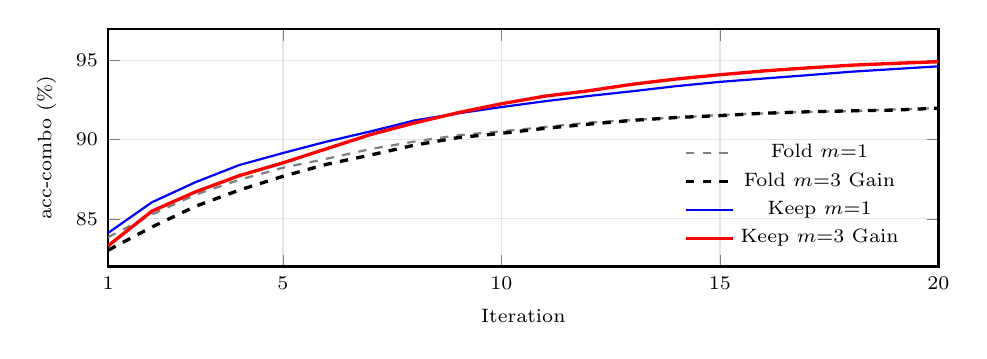
\begin{tikzpicture}
\begin{axis}[
  width=\columnwidth, height=4.6cm,
  xlabel={Iteration}, ylabel={acc-combo (\%)},
  xmin=1, xmax=20, ymin=82, ymax=97,
  xtick={1,5,10,15,20},
  legend pos=south east, legend style={font=\scriptsize, draw=none, fill=none},
  tick label style={font=\scriptsize}, label style={font=\scriptsize},
  grid=major, grid style={gray!20},
  no markers, thick]
\addplot[gray, dashed] coordinates {(1,83.85) (2,85.28) (3,86.53) (4,87.47) (5,88.23) (6,88.80) (7,89.41) (8,89.88) (9,90.28) (10,90.53) (11,90.80) (12,91.08) (13,91.24) (14,91.40) (15,91.56) (16,91.66) (17,91.76) (18,91.80) (19,91.91) (20,91.99)};
\addplot[black, dashed, very thick] coordinates {(1,83.03) (2,84.49) (3,85.80) (4,86.82) (5,87.69) (6,88.45) (7,89.03) (8,89.65) (9,90.13) (10,90.40) (11,90.72) (12,90.98) (13,91.22) (14,91.40) (15,91.52) (16,91.67) (17,91.76) (18,91.82) (19,91.87) (20,91.99)};
\addplot[blue] coordinates {(1,84.12) (2,86.05) (3,87.32) (4,88.40) (5,89.16) (6,89.88) (7,90.52) (8,91.21) (9,91.66) (10,92.06) (11,92.43) (12,92.76) (13,93.06) (14,93.38) (15,93.65) (16,93.86) (17,94.07) (18,94.29) (19,94.46) (20,94.63)};
\addplot[red, very thick] coordinates {(1,83.31) (2,85.49) (3,86.71) (4,87.73) (5,88.54) (6,89.43) (7,90.32) (8,91.05) (9,91.70) (10,92.27) (11,92.75) (12,93.09) (13,93.50) (14,93.83) (15,94.10) (16,94.34) (17,94.53) (18,94.70) (19,94.82) (20,94.92)};
\legend{Fold $m{=}1$, Fold $m{=}3$ Gain, Keep $m{=}1$, Keep $m{=}3$ Gain}
\end{axis}
\end{tikzpicture}
\caption{acc-combo of the learned model after each iteration, mean over the $30$ runs (combination users, all datasets). Dashed: fold; solid: keep; thin: $m=1$; thick: $m=3$ with \textsc{PartitionGain}.}
\label{fig:curve}
\end{figure}

\begin{table}[t]
\centering
\caption{Per dataset (10 runs each): acc-combo (acc-c) and P@10\% (P). Names as in
Table~\ref{tab:main}; Length: score $= |X|$; Offline: models fitted on all pairs of 2000 other patterns,
over items only or items plus the true liked pairs.}
\label{tab:keep_datasets}
\small
\setlength{\tabcolsep}{3.5pt}
\begin{tabular}{lcccccc}
\toprule
& \multicolumn{2}{c}{chess} & \multicolumn{2}{c}{mushroom} & \multicolumn{2}{c}{soybean} \\
\cmidrule(lr){2-3} \cmidrule(lr){4-5} \cmidrule(lr){6-7}
Config. & acc-c & P & acc-c & P & acc-c & P \\
\midrule
Length              & 84.3 & 67.5 & 79.5 & 50.0 & 80.4 & 50.5 \\
LetSIP              & 94.0 & 93.4 & 90.7 & 68.5 & 91.0 & 72.5 \\
Fold $m{=}1$        & 94.5 & 93.6 & 90.5 & 67.7 & 91.0 & 73.8 \\
Fold Gain           & 94.2 & 93.3 & 90.6 & 68.8 & 91.2 & 73.1 \\
Keep $m{=}1$        & 97.2 & 98.8 & 92.8 & 74.2 & 93.9 & 86.2 \\
Keep Top            & 97.8 & 99.3 & 93.8 & 79.3 & 94.3 & 86.4 \\
Keep Gain, 10sw     & 98.4 & 99.4 & 93.6 & 78.9 & 96.1 & 91.8 \\
\midrule
Offline, items      & 94.9 & 99.5 & 91.0 & 69.0 & 93.0 & 78.0 \\
Offline, $+$pairs   & 99.3 & 100  & 97.1 & 87.0 & 98.8 & 96.0 \\
\bottomrule
\end{tabular}
\end{table}

\subsection{Cost and Diversity}
\label{subsec:cost}

Measured with runs executed one at a time (chess), an iteration takes about $2.6$\,s, almost entirely spent sampling the query; the sub-pattern search takes about $35$\,ms over about $70$ distinct candidate covers, every selection rule less than $3$\,ms, and learning and folding about $11$\,ms. Selecting several sub-patterns therefore adds no measurable cost at $k = 10$. Over the last ten iterations, all configurations show the same number of distinct items and the same similarity between shown patterns.


\subsection{Discussion}
\label{subsec:discussion}

Selecting several complementary sub-patterns does not improve preference learning as long as the sub-pattern features are folded into item weights after every iteration: the learner barely uses them, and the folded model cannot represent combinations of items. The bottleneck is therefore the transfer scheme, not the choice of sub-patterns. Once the sub-patterns are kept as features, they improve the model markedly, and several sub-patterns per iteration add a further, smaller gain. Under this scheme, the plain Top rule over distinct covers performs at least as well as partition gain, which suggests that, when features persist across iterations, covering more candidate combinations matters more than complementarity within a single query. These conclusions are limited to $k = 10$, $20$ iterations, item features and synthetic combination users, whose preference has exactly the structure sub-pattern features can express.

\section{Conclusions}
\label{sec:conclusions}

We asked whether preference learning in interactive pattern mining improves when several complementary discriminant sub-patterns, rather than only the strongest one, are used as dynamic features. Within \textsc{DiSPaLe}'s fold-and-discard scheme, the answer is no: every selection rule we studied, including partition gain, leads to the same model as the single best sub-pattern, because the folded model is restricted to item weights and the learner barely uses the temporary features. 

The answer becomes yes once the selected sub-patterns are kept as permanent features: the model then represents preferences for items together, improves significantly on all three datasets, and selecting several sub-patterns per iteration adds a further, smaller gain at no measurable cost.

Along the way, we identified and corrected six errors in the published implementation, made each correction switchable so that its effect can be measured, and verified that undoing all of them reproduces the published code exactly.

Future work should test the keep scheme with real users and with preferences that do not consist of item pairs, limit the growth of the kept feature set, for instance by pruning sub-patterns whose weight stays near zero, and revisit the selection rule under this scheme, where covering many candidate combinations appeared to matter more than complementarity within a single query.


\bibliographystyle{ACM-Reference-Format}
\bibliography{references}

\newpage
\appendix

\section{AI Assistance Disclosure}
We utilized AI as a supportive aid to accelerate our understanding of Java and Scala, languages with which we were previously unfamiliar. This enabled us to comprehend the existing codebase and make the necessary software modifications ourselves. In drafting this report, AI was strictly employed for minor prose refinement and stylistic polishing to ensure clarity and proper academic formatting. All primary concepts, code modifications, data interpretations, and final results remain entirely our own work.

\end{document}
